\section{Risk and Technical Debt}

To measure the risks of this project we will use the following 3x3 risk matrix, which will help us develop the 
\gls{risk assessment}:

\begin{figure}[H]
    \centering
    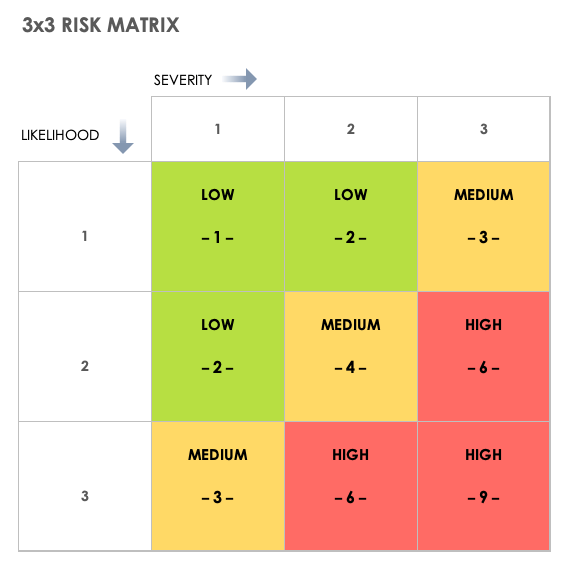
\includegraphics[width=0.5\textwidth]{assets/Risk-Matrix.png}
    \caption{3x3 Risk Matrix Template\\ Source: \citet{refonline:smtrisk}  }
    \label{fig:risk_matrix_template}
\end{figure}


The elements used to identify the risk are shown in the picture below:

\begin{figure}[H]
    \centering
    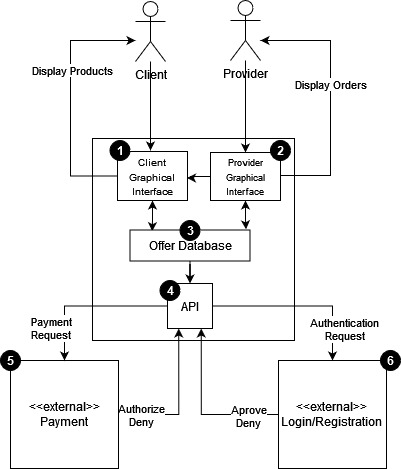
\includegraphics[width=0.4\textwidth]{assets/risk_technical_context.jpg}
    \caption{Modified from Figure \ref{fig:technical_context}}
    \label{fig:risk_technical_context}
\end{figure}

\newpage
The following risk table was defined after several discussion with the team members:

\begin{table}[H]
    \centering
    \resizebox{\textwidth}{!}{%
    \begin{tabular}{|l|llllll}
    %\multicolumn{1}{|c|}{\textbf{{Risk Criteria}} & \multicolumn{6}{|c|}{\textbf{Item}} \\
    \toprule
    \multicolumn{1}{c}{\textbf{Risk Criteria}}              & \multicolumn{6}{c}{\textbf{Element ID}} \\ \hline
    \midrule
    \multicolumn{1}{c}{}              & \multicolumn{1}{c}{\textbf{1}} & \multicolumn{1}{c}{\textbf{2}} & \multicolumn{1}{c}{\textbf{3}} & \multicolumn{1}{c}{\textbf{4}} & \multicolumn{1}{c}{\textbf{5}} & \multicolumn{1}{c}{\textbf{6}} \\ \hline
    \multicolumn{1}{|l|}{\textbf{Unproven technology}}      & \multicolumn{1}{l|}{1} & \multicolumn{1}{l|}{1} & \multicolumn{1}{l|}{1} & \multicolumn{1}{l|}{1} & \multicolumn{1}{l|}{1} & \multicolumn{1}{l|}{1} \\ \hline
    \multicolumn{1}{|l|}{\textbf{Performance}}              & \multicolumn{1}{l|}{2} & \multicolumn{1}{l|}{2} & \multicolumn{1}{l|}{1} & \multicolumn{1}{l|}{1} & \multicolumn{1}{l|}{1} & \multicolumn{1}{l|}{1} \\ \hline
    \multicolumn{1}{|l|}{\textbf{Scalability}}              & \multicolumn{1}{l|}{1} & \multicolumn{1}{l|}{1} & \multicolumn{1}{l|}{2} & \multicolumn{1}{l|}{1} & \multicolumn{1}{l|}{1} & \multicolumn{1}{l|}{1} \\ \hline
    \multicolumn{1}{|l|}{\textbf{Availability}}             & \multicolumn{1}{l|}{1} & \multicolumn{1}{l|}{1} & \multicolumn{1}{l|}{4} & \multicolumn{1}{l|}{2} & \multicolumn{1}{l|}{1} & \multicolumn{1}{l|}{1} \\ \hline
    \multicolumn{1}{|l|}{\textbf{Data loss}}                & \multicolumn{1}{l|}{1} & \multicolumn{1}{l|}{1} & \multicolumn{1}{l|}{3} & \multicolumn{1}{l|}{1} & \multicolumn{1}{l|}{1} & \multicolumn{1}{l|}{1} \\ \hline
    \multicolumn{1}{|l|}{\textbf{Single points of failure}} & \multicolumn{1}{l|}{1} & \multicolumn{1}{l|}{1} & \multicolumn{1}{l|}{4} & \multicolumn{1}{l|}{4} & \multicolumn{1}{l|}{1} & \multicolumn{1}{l|}{1} \\ \hline
    \multicolumn{1}{|l|}{\textbf{Security}}                 & \multicolumn{1}{l|}{1} & \multicolumn{1}{l|}{2} & \multicolumn{1}{l|}{3} & \multicolumn{1}{l|}{2} & \multicolumn{1}{l|}{2} & \multicolumn{1}{l|}{2} \\ \hline
    \bottomrule
\end{tabular}%
    }
\end{table}

\textbf{}

\subsection{Motivation}

\begin{table}[H]
    \setstretch{1.0}
        \begin{tabularx}{\textwidth}{|l|X|X|X|}
        \toprule
           \textbf{Risk Criteria} & \textbf{1 Client Graphical Interface} & \textbf{2 Provider Graphical Interface} & \textbf{3 Offer Database} \\
        \midrule
        \textbf{Unproven technology}& \textit{not applicable} & \textit{not applicable} & \textit{not applicable} \\
        \hline
        \textbf{Performance} & Concerns regarding a such dynamic shop. Data displayed & Concerns regarding a such dynamic shop. Data update. & \textit{not applicable} \\
        \hline
        \textbf{Scalability} & \textit{not applicable} & \textit{not applicable} & One database can be overwhelmed if the number of user is not limited for this prototype version. \\
        \hline
        \textbf{Availability} & \textit{not applicable} & \textit{not applicable} & In case of intense traffic the latency can be more than expected. \\
        \hline
        \textbf{Data loss} & \textit{not applicable} & \textit{not applicable} & Nowadays no company can survive in case of data loss. Technical damages can be 
        mostly easy fixed, but moral damage stays forever. \\
        \hline
        \textbf{Single points of failure} & \textit{not applicable} & \textit{not applicable} & Only one component gives always this risk. Increasing the 
        number of components increases also the total development costs \\
        \hline
        \textbf{Security} & \textit{not applicable} the client's input is always processed
        by the API and by the third party providers & If no strong data filtering exists, providers can upload
        malicious files or execute unwished commands. & The filtering of the input should occur mostly on the server side, Source
        no external access can figure out, how it is implemented. \\
        \bottomrule
    \end{tabularx}
\end{table}

\begin{table}[H]
    \setstretch{1.0}
    \begin{tabularx}{\textwidth}{|l|X|X|X|}
        \toprule
        \textbf{Risk Criteria} & \textbf{4 API} & \textbf{5 External Payment Service} & \textbf{6 External Authentication Service} \\
        \midrule
        \textbf{Unproven technology} & \textit{not applicable} & \textit{not applicable}  & \textit{not applicable}  \\
        \hline
        \textbf{Performance} & \textit{not applicable} & \textit{not applicable}  & \textit{not applicable} \\
        \hline
        \textbf{Scalability} & \textit{not applicable} & \textit{not applicable} & \textit{not applicable} \\
        \hline
        \textbf{Availability} & The access to the products become unstable. & \textit{not applicable} & \textit{not applicable} \\
        \hline
        \textbf{Data loss} & \textit{not applicable} & \textit{not applicable} & \textit{not applicable} \\
        \hline
        \textbf{Single points of failure} & In case of failure login, registration and payment are compromised. & \textit{not applicable} & \textit{not applicable} \\
        \hline
        \textbf{Security} & Lack of practical experience within the team about this topic. we rely on the service provided by the third party companies 
        & SLA Less than 99.5\% but equal to or greater than 95.0\% \cite{refmisc:paycSLA} & SLA < 99.99\% - >= 99.9\% \cite{refmisc:auth0sla}	\\
        \bottomrule
    \end{tabularx}
\end{table}
%1 - 
%